\documentclass[11pt, fleqn]{article}
\usepackage{graphicx}
\usepackage{a4wide}
\usepackage{float}
\usepackage[top=3cm,bottom=3cm,left=2.5cm,right=2.5cm]{geometry}
\usepackage{algorithm}
\usepackage{listings}
\pagenumbering{arabic}

%kodovani vstupu
\usepackage[utf8]{inputenc}%latin2,windows-1250
%podpora pro specificke znaky, napr. ceske
\usepackage[T1]{fontenc}
%podpora pro ceske deleni slov atd.
\usepackage[czech]{babel}

%dalsi moznosti zarovnani sloupcu v tabulkach
\usepackage{array}
%vkladani obrazku
\usepackage{graphicx}
\usepackage{wrapfig}
\usepackage{subfig}
\usepackage{color}
\usepackage[table,xcdraw]{xcolor}


\setlength{\parindent}{1em}
\setlength{\parskip}{0.8em}
\pdfminorversion=6

\lstset{language=C++,basicstyle=\footnotesize\ttfamily,
  morekeywords={\#pragma},
  keywordstyle=\color{red},
  stringstyle=\color{red},
  commentstyle=\color{gray},
  tabsize=2,
  frame=none,
  numbers=left,
  xleftmargin=2em,
}

\title{Hledání nejkratších cest v grafu \\ MI-PRC ZS2017/2018}
\author{Jakub Kulík \& Martin Piták}

\begin{document}
\maketitle

\section{Úvod}

Hledání nejkratších cest v grafu je relativně častý problém a proto na něj vzniklo nemalé množství efektivních algoritmů (v závislosti na ocenění cest a jejich oboustrannosti). Níže jsou popsané dva algoritmy na nalezení nejkratších cest mezi všemi dvojicemi bodů v grafu. Jeden z nich je Dijkstrův algoritmus spuštěný z každého bodu a druhý je efektivnější Floyd-Warshall algoritmus.

Přiložená implementace čte grafy s unifikovanou cenou cesty 1, nicméně implementace algoritmů samotných umí bez jakékoliv změny pracovat i s jinou cenou hran.

\section{Dijkstrův algoritmus}

Dijkstrův algoritmus slouží pro nalezení nejkratších cest v~grafu pro jeden vrchol grafu.

Algoritmus pracuje s~maticí přechodů, která neobsahuje záporné hrany.

\subsection{Implementace Dijkstrova algoritmu}
Základní verze algoritmu je velmi jednoduchá a přímočará. Pro dvoudimenziovální matici sousednosti nám stačí tři for cykly a jeden if.

Algoritmus pracuje nad maticí vzdáleností, která má na začátku všechny vzdálenosti (kromě těch již známých) nastavené na nekonečno. Do této matice víše popsaným algoritmem postupně dopsisuje dopočítané vzdálenosti. Takto postupně zvětšuje počet meziuzlů (celkem $n$ krát, kde $n$ je počet uzlů v grafu), až dopočítá všechny možné cesty mezi uzly.

\subsection{OpenACC version}
OpenACC verze algoritmu se neliší téměř vůbec od verze sekvenční - jediným rozdílem je přidání několik \lstinline{#pragma}.

\lstinline{#pragma acc data copy(dm[0 : size][0 : size])}, zajistí překopírované dat na grafickou kartu a zase zpátky.

\lstinline{#pragma acc parallel} určuje block běžící na grafické kartě.

\lstinline{#pragma acc loop independent} říká acc, že jednotlivé běhy následujícího for cyklu jsou na sobě nezávislé a proto se mohou paralelizovat.

\lstinline{#pragma acc loop} říká acc, že následující for cyklus se má paralelizovat a že si sám má zjistit zavislosti.


\subsection{měření OpenACC verze programu}

Měření Dijkkstrova algoritmu jsou pro CPU provedeny na Intel Core i5-5200U CPU (dvě jádra s HyperThreadingem - 2.2GHz, až 2.7GHz with TurboBoost) s 16GB DDR4 RAM. GPU použité u OpenACC verzí je nVidia GeForce 480 na školním serveru star. Matice (grafy) použité pro všechna měření jsou náhodně generovány generátorem přiloženém k našemu zadání. Matice jsou velikostí 100 až 2500 s průměrným stupněm uzlu 30.

Měření na každém grafu je provedené třikrát a použité jsou zprůměrované hodnoty.

\begin{figure}
  \centering
  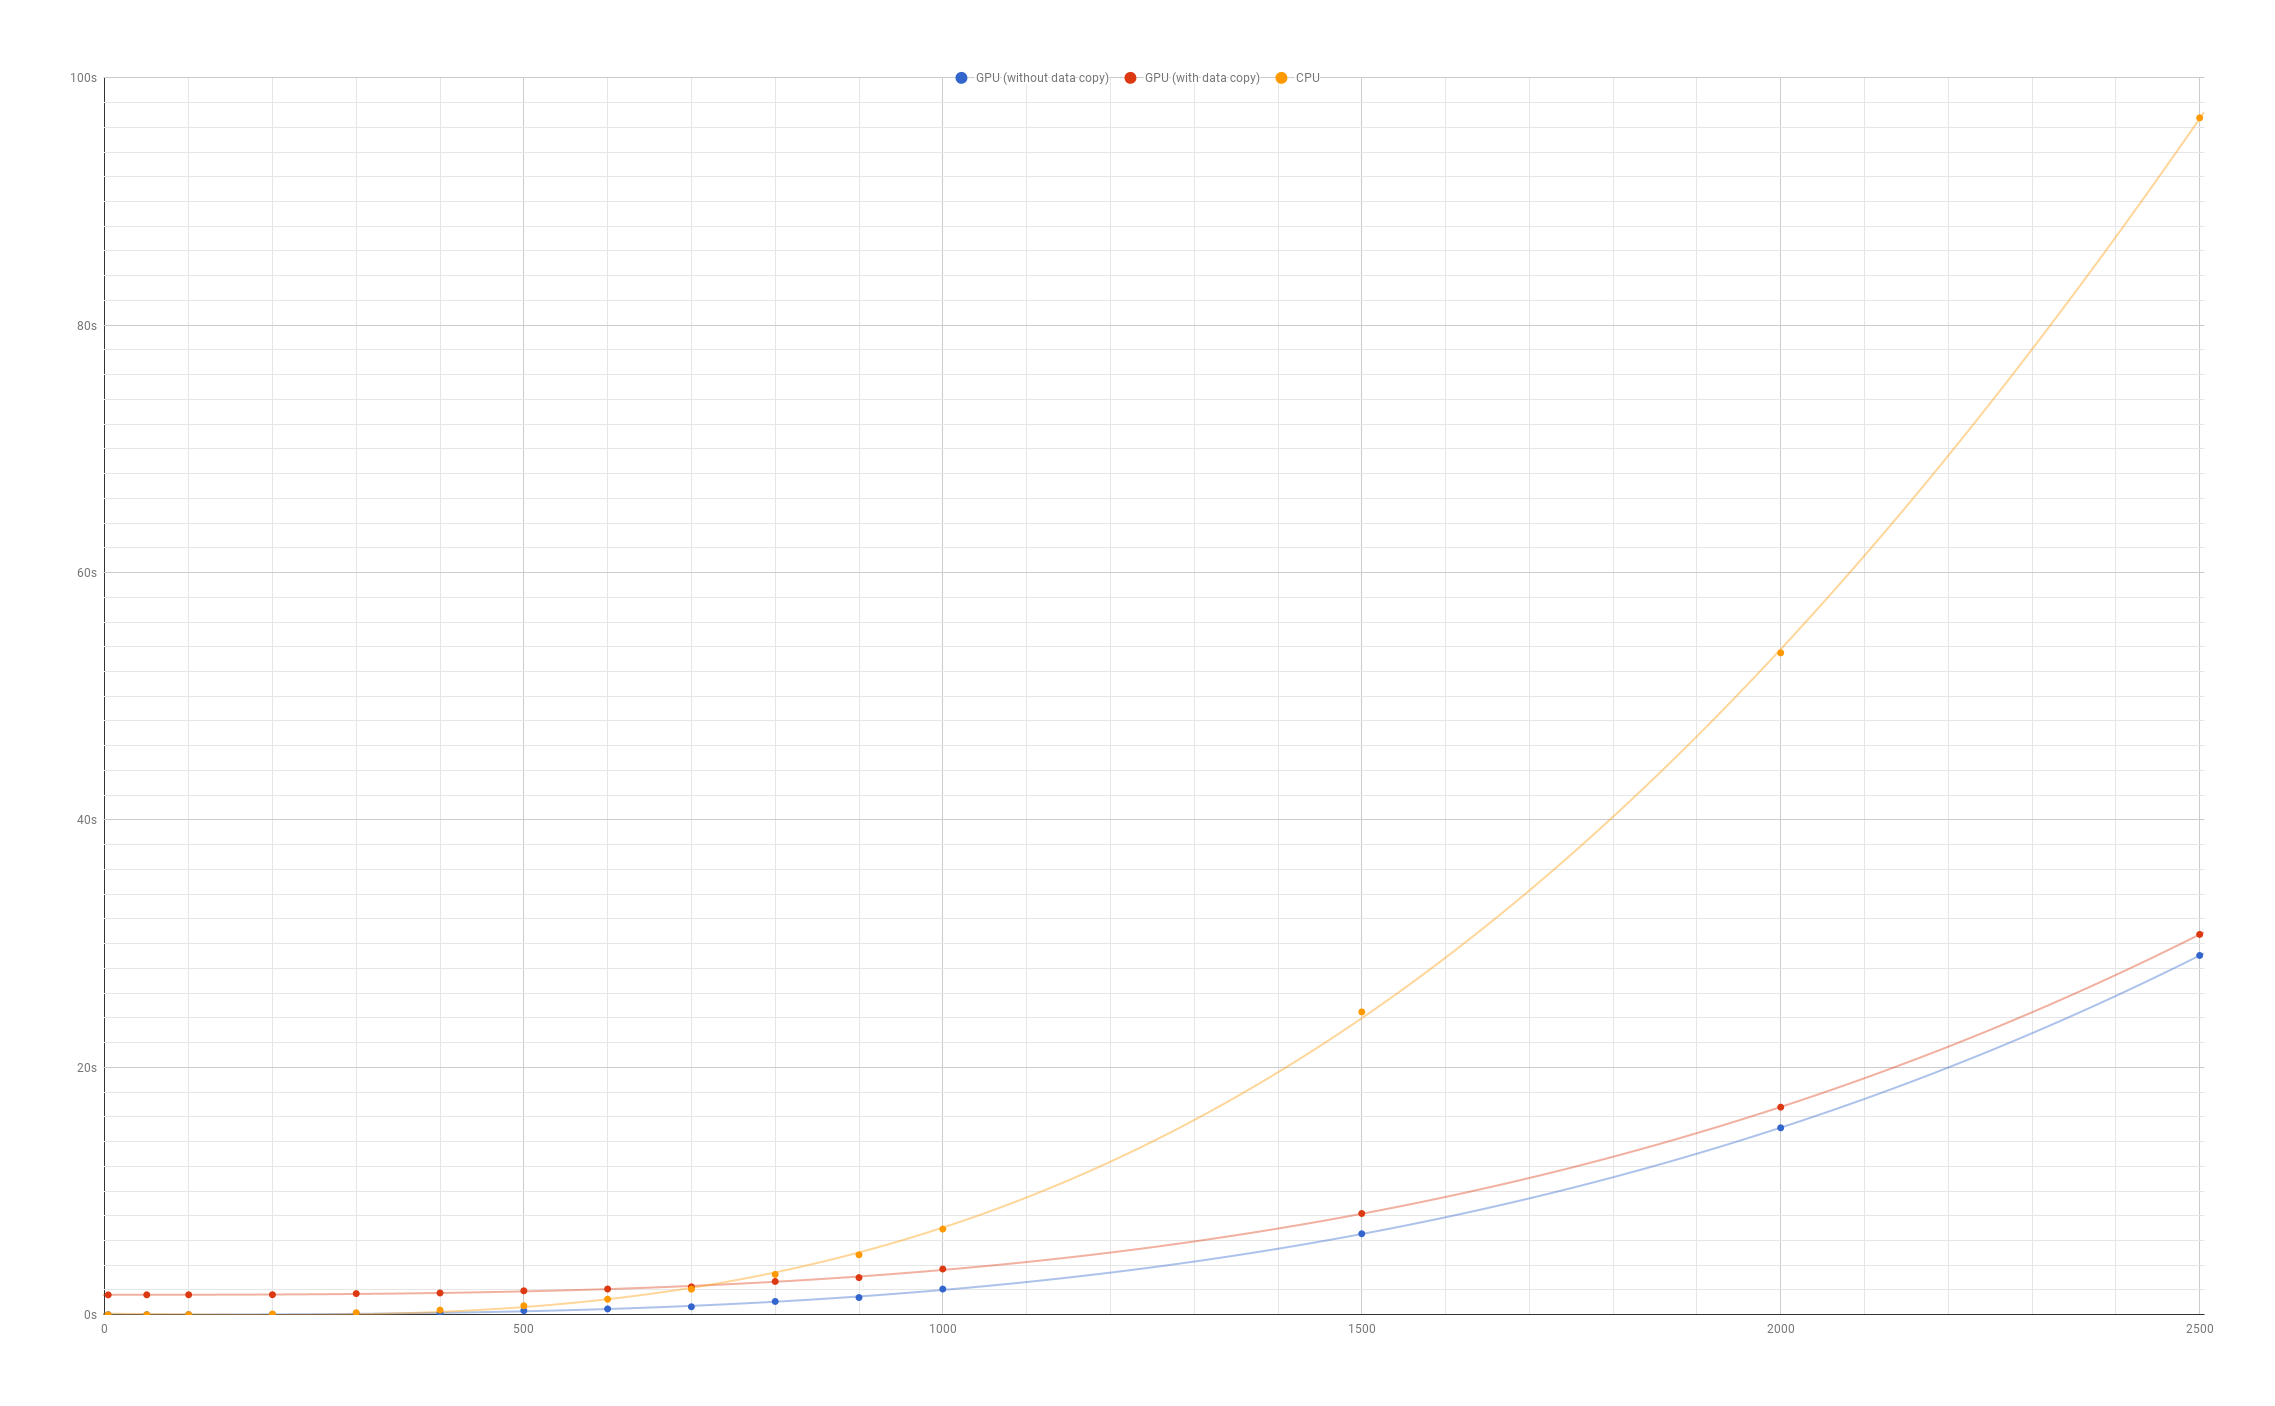
\includegraphics[width=.7\linewidth]{../results/Dijkstra.png}
  \captionof{figure}{Porovnání Dijkstry na CPU a přes OpenACC}
  \label{fig:d1}
\end{figure}

Poznámka: Průměrná stupeň uzlu grafu nemá na algoritmus žádný vliv, protože se stejně prochází postupně všechny iterace bez ohledu na to, jak samotný graf vypadá. Jediný malý rozdíl může být v přípdě velmi řídkých grafů, kde budu minimálně zapisovat do paměti, nicméně to pro nás zde není podstatné.

Z naměřených dat je vidět, že zrychlení není až tak velké jak by se očekávalo. U menších velikosti grafů (do 1000) je vidět že kopírování dat trvá déle než samotný výpočet a také, že kopírování je je přibližně vždy stejné a nezávísí tolik na velikosti matice. Dálě je z grafu vidět, že CPU verze je pro menší instance rychlejší a to hlavně z toho důvodu, že režie spouštění kernelu a nakopírování dat na grafické kartě převyšuje zisky nasledně velmi rychlého kernelu (viz. graf \ref{fig:d1}).


\subsection{Cuda version}

Cuda verze programu pracuje se stejným algoritmem jako OpenACC verze. Jediná změna bylo, že jsem použil memset na alokaci pole, v dokumentaci jsem si prečetl, že memset se chová podoběn jako samostaný kernel. Chtěl jsem použít volnání kernelu v kernelu ale když jsem narazil na bararieru kdy bych musel předávat všechny proměné. A také bariera s contextem proměných.

\subsection{měření Cuda verze programu}

Veškerá měření jsou ze školního serveru star (GPU nVidia GeForce GTX 480). Matice (grafy) použité pro všechna měření jsou náhodně generovány generátorem přiloženém k našemu zadání. Matice jsou velikostí 100 až 2500 s průměrným stupněm uzlu 30.

Měření na každém grafu je provedené třikrát a použité jsou zprůměrované hodnoty.

Z naměřených hodnot je vidět, že nejvice trvá kopirování dat mezi CPU a GPU. Doba běhu roste podle očekávání polynomiálně.

I přesto se nepodařilo implementovat takový algoritmus, který by se dokázal vyrovnat OpenACC verzi\ref{fig:d1}. Důvodem může být jiná implementace, ACC verze a jiný způsob měření. Kromě toho, že v OpenACC verzi se měřilo přes \lstinline{omp_get_wtime()} a v Cuda verzi přes \lstinline{clock()}, byli úlohy i jinak spouštěné. Další důvod pro pomalejší běh může být také to, že OpenACC se podařilo zparalelizovat některe vnořené cykly. Na grafu\ref{fig:d2} je vidět jak, i zde ma kopirovaní matice relativně konstatni přírustek.

\begin{figure}
  \centering
  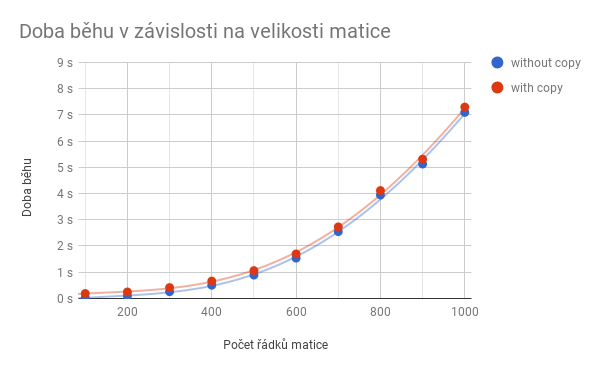
\includegraphics[width=.7\linewidth]{../results/cuda_dijkstra.png}
  \captionof{figure}{Graf doby běhu Dijkstry na na GPU přes cudu}
  \label{fig:d2}
\end{figure}

\section{algoritmus Floyd-Warshall}

Floyd–Warshall algoritmus je algoritmus pro nalezení nejkratších cest v orientovaném grafu. Algoritmus v každé iteraci zkusí pro všechny dvojice uzlů nalézt nejkratší cestu mezi dvěmi úhly. To dělá postupně $n$ krát, takže všechny existující cesty jsou postupně dopočítány. Každou iterací se zvětšuje množství uzlů přes, přes které se mezi dvojicí uzlů dostanu. Při poslední iteraci tak uvažuji i cestu přes všechny uzly v grafu. Pokud cesta mezi hranami existuje, bude na jejím místě v matici vzdáleností správná vzdálenost. Pokud cesta neexistuje, hodnota bude nastavená na nekonečno.

Vzhledem k tomu, že se využívá matice sousednosti, nedá se algoritmus použít pro multi grafy. Algoritmus nemá problémy se záporně ohodnocenými hranamy, vrací ale nesprávné výsledky, pokud existují záporně ohodnocené cykly.


\subsection{Implementace Floyd Warshall algoritmu}
Základní verze algoritmu je velmi jednoduchá a přímočará. Pro dvoudimenziovální matici sousednosti nám stačí tři for cykly a jeden if.

Algoritmus pracuje nad maticí vzdáleností, která má na začátku všechny vzdálenosti (kromě těch již známých) nastavené na nekonečno. Do této matice víše popsaným algoritmem postupně dopsisuje dopočítané vzdálenosti. Takto postupně zvětšuje počet meziuzlů (celkem $n$ krát, kde $n$ je počet uzlů v grafu), až dopočítá všechny možné cesty mezi uzly.


\subsection{OpenACC version}
OpenACC verze algoritmu se neliší téměř vůbec od verze sekvenční.

OpenACC verze se ve skutečnosti liší relativně hodně, protože potřebuje lehce přeskládat pořadí provádění a tedy změnit algoritmus. Tzv. blocked algoritmus rozdělí celou matici na bloky (v našem případě o velikosti 1x1) a poté pro každý blok na diagonále nejprve spočíta fw pro řádek a sloupec (ve kterém blok je) s $k$ nastaveným na blok a poté dopočítá všechny ostatní ($k$ je opět nastavené na blok). Tímto způsobem můžeme paralelizovat jednotlivé části bez problémů se synchronizací.

Pro optimálnější běh algoritmu jsou oba dva for cykly pro řádky a sloupce sjednocené do jednoho kernelu a předpočítány pro celou matici (pro každý blok na diagonále). Nicméně tato část je relativně výpočetně nenáročná a proto není důležitá. Hlavní část má paralelizované dva cykly - pro každý blok se kernel spouští znovu z důvodu časových závislostí. V naši implementaci počítá poslední část opět úplně všechna pole a ne jen ta nedopočítaná. Důvoduem je, že přidávání podmínek by nedělalo paralelnímu provádění moc dobře a zbytečně by ho zpomalovalo. Dopočítat znovu všechno (již vypočítané bloky se druhým průchodem nezmění) nám zajistí rychlejší provedení. Zároveň se jedná jen o malou část výpočtu a není s ní tedy moc problém.

\lstinline{#pragma acc data copy(dm[0 : size][0 : size])}, zajistí překopírované dat na grafickou kartu (kompilátor ji přidá, pokud není explicitně zadána).

\lstinline{#pragma acc parallel num_gangs(1024) vector_length(128)} určuje block běžící na grafické kartě s explicitně zadanými velikostmi gangů a vektoru.

\lstinline{#pragma acc loop collapse(2)} říká acc, že následující for cyklus se má paralelizovat a že následující dva for cykly složené do jednoho.


\subsection{měření OpenACC verze programu}

Měření Floyd Warshallova algoritmu jsou pro CPU provedeny na Intel Core i5-7200U (dvě jádra s HyperThreadingem - 2.5GHz, až 3.1GHz with TurboBoost) s 8GB DDR4 RAM. GPU použité u OpenACC verzí je nVidia GeForce 480 na školním serveru star. Matice (grafy) použité pro všechna měření jsou náhodně generovány generátorem přiloženém k našemu zadání. Matice jsou velikostí 100 až 2500 s průměrným stupněm uzlu 30.

Měření na každém grafu je provedené třikrát a použité jsou zprůměrované hodnoty.

\begin{figure}
  \centering
  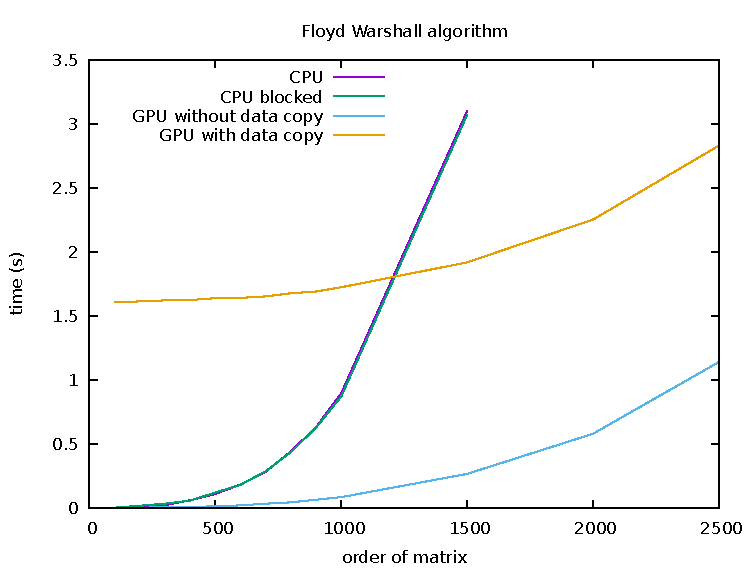
\includegraphics[width=.7\linewidth]{../results/Floyd_Warshall.pdf}
  \captionof{figure}{Porovnání různách verzí Floyd Warshalla}
  \label{fig:fw1}
\end{figure}

Poznámka: Průměrná stupeň uzlu grafu nemá na algoritmus žádný vliv, protože se stejně prochází postupně všechny iterace bez ohledu na to, jak samotný graf vypadá. Jediný malý rozdíl může být v přípdě velmi řídkých grafů, kde budu minimálně zapisovat do paměti, nicméně to pro nás zde není podstatné.

Z naměřených dat je vidět, že většina času výpočtu na grafické kartě je zabraná kopírováním dat z a do grafické karty. Samotný výpočet je z pravidla pouze zlomkem času. Další věcí, která je vidět z grafů je, že CPU verze je pro menší instance rychlejší a to hlavně z toho důvodu, že režie spouštění kernelu na grafické kartě převyšuje zisky nasledně velmi rychlého kernelu (viz. graf \ref{fig:fw1}). V grafu jsou vidět obě verze sekvenčního algoritmu, které jsou výkonostně srovnatelné (i přesto, že block verze počítá také některé hodnoty dvakrát).

Pro nalezení optimálního nastaení algoritmu bylo vyzkoušeno několik různých konfigurací počtu gangů a velikostí vektorů nad grafem o velikosti 1000 (viz. tabulka \ref{fig:fw2}). Z výsledné tabulky je vidět, že příliš malé vektory způsobují veliké zpomalení algoritmu (velikost 512 není již v tabulce, nicméně algoritmus tam opět zpomaluje). Počet gangů nemění performace algoritmu tolik.

Pro větší grafy se tato čísla mohou lišit a proto je třeba optimální nastavení vždy hledat pro konkrétní velikosti grafů.

Pozorování: Pokud se zadá velikost vektoru například 65535, vypíše kompilátor, že jsou vektory moc veliké a ignoruje je tedy, nicméně výsledný kód je stále o dost zrychlený a to až 100krát oproti vektorům velikosti 128. Nicméně výsledky jsou poté občas opět špatně. 

\begin{table}[tbp]
  \centering
  \caption{Výkon dle velikosti vektoru a počtu gangů}
  \label{fig:fw2}
  \def\arraystretch{2}
  \begin{tabular}{llccccc}
    gangs / vector\_size & 16 & 32 & 64 & 128 & 192 & 256 \\
    \rowcolor[HTML]{ECF4FF} 
    128  & 0.5910 & 0.3179 & 0.1677 & 0.1103 & 0.1107 & 0.0936 \\
    192  & 0.4042 & 0.2175 & 0.1143 & 0.0916 & 0.1011 & 0.0919 \\
    \rowcolor[HTML]{ECF4FF} 
    256  & 0.4566 & 0.2440 & 0.1251 & 0.0941 & 0.0975 & 0.0941 \\
    512  & 0.4457 & 0.2480 & 0.1286 & 0.9391 & 0.0924 & 0.0911 \\
    \rowcolor[HTML]{ECF4FF} 
    1024 & 0.4118 & 0.2228 & 0.1165 & 0.0905 & 0.0915 & 0.0901 \\
    2048 & 0.4116 & 0.2272 & 0.1183 & 0.0900 & 0.0903 & 0.0896
  \end{tabular}
\end{table}

\subsection{Cuda version}

Cuda verze programu pracuje s blocked verzí původního algoritmu stejně jako OpenACC verze. Bloky mají fixní velikost 32x32, díky čemuž se vejdou do maximálního počtu vláken na Cuda block.

První tři kernely (pro independent a n-aligned bloky) zabírají minimální procento celého výpočetního času a proto nebyli nijak optimalizovány. Jejich implementace je velmi přímočará a kromě načtení pozice a ověření okrajů matice už pouze počítají jim dané políčko matice.

Pro dvojzávislé bloky jsou v implementaci celkem čtyři různé kernely. První je opět přímočarou Cuda implementací blocked verze. Používá \lstinline{dim3} struktury pro bloky i vlákna tak, aby pokryl celou matici. Také jako jediný má $k$ cyklus před voláním kernelu a ne v něm.

Druhý kernel je velmi podobný, jen nechává jedno vlákno zpracovat celý řádek jednoho bloku. Dále také přesouvá $k$ dovnitř do kernelu.

Třetí implementace kopíruje svůj blok z globální paměti do \lstinline{shared} a výpočty provádí nad sdílenou a rychlou pamětí. Každé vlákno nejprve překopíruje jedno svoje políčko a potom nad ním počítá pro všechna $k$. Po dokončení výpočtu se opět kopíruje zpět do globální paměti.

Poslední implementace spojuje oba dva předchozí přístupy dohromady a pracuje nad sdílenou pamětí s méně vlákny dělajícími více práce.

\subsection{měření Cuda verze programu}

Veškerá měření jsou ze školního serveru star (GPU nVidia GeForce GTX 480). Matice (grafy) použité pro všechna měření jsou náhodně generovány generátorem přiloženém k našemu zadání. Matice jsou velikostí 100 až 2500 s průměrným stupněm uzlu 30.

Měření na každém grafu je provedené třikrát a použité jsou zprůměrované hodnoty.

Z prvního grafu je zřetelné, že verze s vlákny dělajícími více práce jsou výrazně horší než dvě druhé \ref{fig:fw3}. To je pravděpodobně zapříčeněné overheadem z cyklů v každém vlákně. Počet vláken na blok je přesně o velikosti warpu (takže tam by problém být neměl), je ale možné, že omezení rezidentních bloků způsobuje výpadky z důvodu latence.

Verze s velmi naivní reimplementací do Cuda dosahuje relativně dobrých výsledků a u menších matic se dá srovnávat s verzí se shared memory, která je dle grafu zdaleka nejlepší a už pro 2000 prvků je i s kopírováním dat rychlejší, než gvýpočet všech ostaních \ref{fig:fw4}. 

I přesto se nepodařilo implementovat takový algoritmus, který by se dokázal vyrovnat OpenACC verzi\ref{fig:fw5}. Důvodem může být jiná implementace ACC verze a jiný způsob měření. Kromě toho, že v OpenACC verzi se měřilo přes \lstinline{omp_get_wtime()} a v Cuda verzi přes \lstinline{clock()}, byli úlohy i jinak spouštěné. OpenAcc verze byla spouštěná plánovačem, Cuda verze přímo (z důvodu nefunkčnosti plánovače).

\begin{figure}
  \centering
  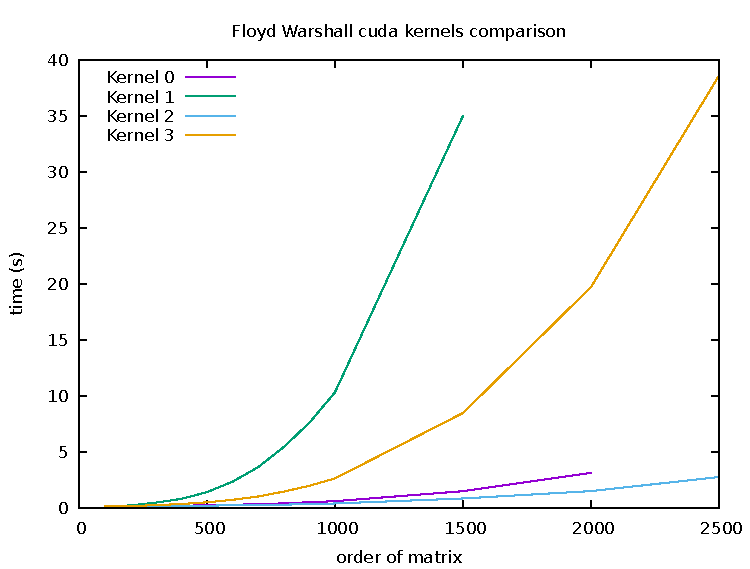
\includegraphics[width=.7\linewidth]{../results/FW_Cuda.pdf}
  \captionof{figure}{Základní porovnání všech kernelů}
  \label{fig:fw3}
\end{figure}

\begin{figure}
  \centering
  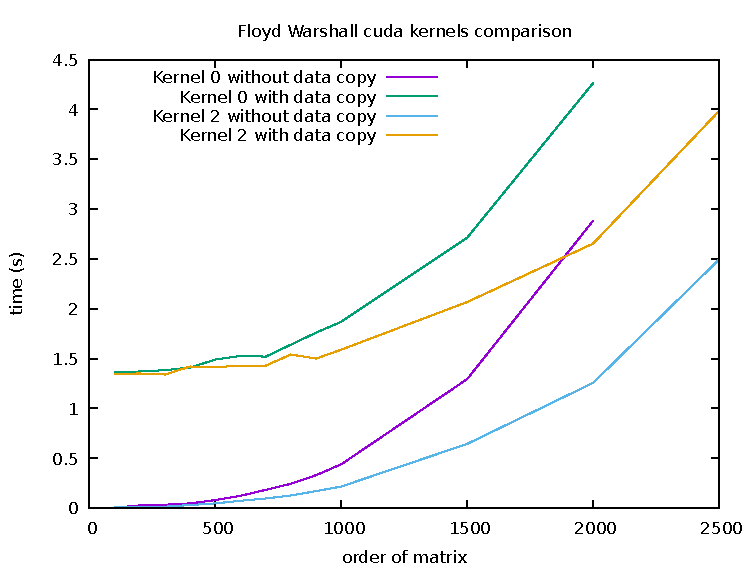
\includegraphics[width=.7\linewidth]{../results/FW_Cuda2.pdf}
  \captionof{figure}{Porovnání dvou nejlepších kernelů}
  \label{fig:fw4}
\end{figure}


\begin{figure}
  \centering
  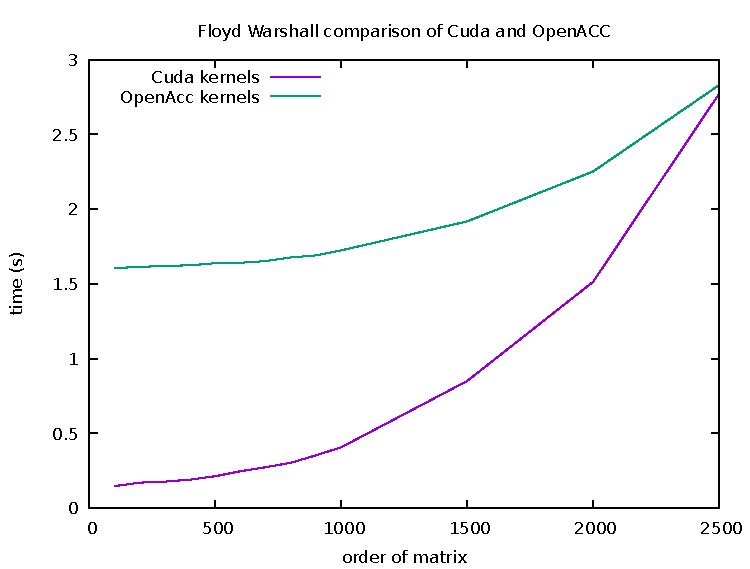
\includegraphics[width=.7\linewidth]{../results/FW_Cuda3.pdf}
  \captionof{figure}{Porovnání Cuda \& OpenAcc verze}
  \label{fig:fw5}
\end{figure}



\end{document}
